% Manuscript in the Nature Scientific Reports layout (wlscirep.cls, single column). Compile on Overleaf with
% pdfLaTeX + BibTeX; the class sets the bibliography style (naturemag-doi.bst) and needs jabbrv.sty with its .ldf files.
% Same text and numbers as the IEEE version (main_source.tex), with the sections in Scientific Reports order.
% Every number in the tables is generated from saved results by src/make_paper_tables.py;
% figures by src/make_paper_figures.py. Affiliations are placeholders (to be completed by the authors).
\documentclass{wlscirep}
\graphicspath{{figures/}{./}} % figures/ locally; project root on Overleaf

\title{Rendering gain and sequence modeling in 12-lead ECG-image classification: a controlled comparison with external validation}

\author[1]{Miriam Istanboli}
\author[2,*]{Mohamed Yousry Elgendi}
\affil[1]{[Affiliation to be added]}
\affil[2]{[Affiliation to be added]}
\affil[*]{Corresponding author: [e-mail to be added]}

\keywords{Electrocardiography, ECG images, deep learning, external validation, shortcut learning, vision transformer, temporal convolutional network, PTB-XL}

\begin{abstract}
Many electrocardiograms (ECGs) exist only as paper, scans or PDFs, yet image classifiers are rarely compared under controlled conditions, and rendering choices are seldom examined. We rendered all 21{,}388 labeled 12-lead PTB-XL records as calibrated paper-style pages and compared five heads on one shared convolutional encoder (column pooling, a capacity-matched per-column network without sequence mixing, an LSTM, a temporal convolutional network and a small vision transformer), each with five seeds, plus a signal reference. On the test fold, capacity explained most of the gain over pooling (0.035 macro AUROC), but heads relating information along each lead row added 0.011--0.020 (Holm-adjusted $p\le0.02$). The renderer lowered page gain for high-voltage ECGs, encoding amplitude, and hence hypertrophy, in the layout and calibration pulse; integrated gradients and a pulse intervention showed whole-row models reading the pulse as a voltage scale. Re-rendering every page at one fixed gain never reduced performance and helped local models most (CNN-only: $+0.030$ macro, $+0.073$ hypertrophy AUROC). Both findings were confirmed, under a prespecified, frozen analysis plan, on external cohorts from the USA ($n=6{,}047$) and China ($n=9{,}004$), where fixed gain improved hypertrophy AUROC for every architecture. Gain policy is a first-order design variable and should be fixed and reported.
\end{abstract}

\begin{document}

\flushbottom
\maketitle
\thispagestyle{empty}

\section*{Introduction}
The 12-lead electrocardiogram (ECG) is the most widely used cardiac test, and deep neural networks trained on digital ECG signals now match or exceed expert performance for many diagnostic statements \cite{hannun2019cardiologist,ribeiro2020automatic,strodthoff2021benchmark,siontis2021ai}. In routine care, however, a large share of ECGs is stored or exchanged as printouts, scans, photographs or image-only PDFs. Methods that classify ECG \emph{images} directly \cite{sangha2022images}, or first digitize them back into signals \cite{reyna2024challenge,krones2024hough}, are therefore of practical interest, and synthetic page renderers have become a standard way to create large labeled image datasets from public signal databases \cite{shivashankara2024ecgimagekit}.

Two questions are rarely controlled in this literature. First, architectural comparisons usually change the feature extractor, the model size and the training recipe at the same time, so it is unclear whether gains from recurrent, convolutional-sequence or attention-based heads reflect sequence modeling or simply more parameters. Second, the rendering policy that turns a signal into a page is treated as a technical detail. Clinical ECGs are printed at a standard gain of 10~mm/mV with a 1-mV calibration pulse \cite{kligfield2007standardization}, but printers and renderers commonly reduce the gain when large deflections would overlap neighboring leads. Because QRS amplitude is itself a diagnostic criterion for ventricular hypertrophy \cite{sokolow1949lvh}, an amplitude-dependent gain policy can leak diagnostic information into the page layout. Such dataset artifacts are a known source of shortcut learning in medical imaging \cite{geirhos2020shortcut,degrave2021covid,zech2018pneumonia}.

\emph{Signal-domain ECG classification.} Convolutional networks on raw ECG signals perform strongly on large cohorts \cite{hannun2019cardiologist,ribeiro2020automatic}. On PTB-XL, a benchmark of signal models reported macro AUROCs around 0.93 for the five diagnostic superclasses, with one-dimensional residual networks among the best \cite{strodthoff2021benchmark,wang2017timeseries}. The PhysioNet/Computing in Cardiology Challenges 2020 and 2021 pooled several international 12-lead databases and showed how heterogeneous labels and populations complicate generalization \cite{perezalday2020challenge,reyna2021challenge,reyna2022issues}.

\emph{ECG images.} Sangha \emph{et al.} trained convolutional networks on ECG images and signals for multilabel diagnosis \cite{sangha2022images}. ECG-Image-Kit generates synthetic paper ECGs from signals \cite{shivashankara2024ecgimagekit}, and the George B. Moody PhysioNet Challenge 2024 addressed digitization and classification of ECG images \cite{reyna2024challenge,krones2024hough}. These works vary the visual appearance of pages but do not, to our knowledge, isolate the effect of the gain policy on classification.

\emph{Sequence heads and evaluation.} Recurrent networks \cite{hochreiter1997lstm}, temporal convolutional networks \cite{bai2018tcn} and transformers \cite{vaswani2017attention,dosovitskiy2021vit} are common choices for aggregating features along time or image width. Model comparisons are sensitive to training variance \cite{bouthillier2021variance} and to repeated use of a test set \cite{varoquaux2022failures}; we therefore report every seed and treat the reused PTB-XL test fold as exploratory, with an untouched external test as confirmation. Reporting follows the spirit of TRIPOD+AI \cite{collins2024tripodai}.

We address both questions in a controlled study with prospectively specified protocols on PTB-XL \cite{wagner2020ptbxl}, with confirmation on two independent cohorts. Our contributions are:
\begin{enumerate}
\item A controlled comparison of five classification heads on one shared convolutional encoder, including a \emph{capacity-matched} head that cannot relate positions along a lead row, so that the benefit of sequence modeling is separated from head capacity. Every network is trained with five seeds, and pairwise differences are assessed with a hierarchical seed-by-patient bootstrap and Holm correction.
\item The identification and mechanistic analysis of an adaptive-gain rendering cue, using gain-stratified prevalence, test-time re-rendering, integrated gradients and a calibration-pulse intervention.
\item A gain-controlled re-rendering that improves every architecture, and an external confirmatory test on cohorts from the USA and China, performed once under a frozen analysis plan.
\item A signal-domain reference that quantifies the cost of the image representation, and a fully reproducible pipeline with hash-bound run records.
\end{enumerate}

\section*{Results}

\subsection*{Controlled head comparison on PTB-XL}
Table~\ref{tab:ptbxl} and Fig.~\ref{fig:heads} (left) summarize the test-fold results. With adaptive gain, macro AUROC rose from 0.830 for the CNN-only head to 0.865 for the capacity-matched head and to 0.876--0.886 for the three sequence heads. Capacity alone accounted for $+0.035$ [0.029, 0.042] (Table~\ref{tab:pairs}). Each sequence head outperformed the capacity-matched head after Holm correction ($+0.011$ to $+0.020$), on validation as well as test and in the GPU-only seed set. The three sequence heads were not separable on the test fold: ViT minus temporal convolution $+0.006$ [$-$0.001, 0.013], adjusted $p=0.17$. The seed-to-seed standard deviation (0.003--0.007) was of the same order as several between-head differences, underlining the need for multiple seeds. The signal-domain reference reached 0.928 $\pm$ 0.001, consistent with published superclass benchmarks \cite{strodthoff2021benchmark}, and exceeded the best image models by 0.03--0.04.

\begin{table}[!t]
\centering
\caption{PTB-XL test fold (exploratory): mean over seeds 42--46 (mean $\pm$ SD for macro AUROC).}
\label{tab:ptbxl}
\footnotesize
\begin{tabular}{llcccccccc}
\toprule
Pages & Model & Macro AUROC & Macro AP & Macro F1 & NORM & MI & STTC & CD & HYP \\
\midrule
Adaptive & CNN-only & 0.830 $\pm$ 0.004 & 0.625 & 0.490 & 0.887 & 0.795 & 0.868 & 0.811 & 0.789 \\
Adaptive & CNN-only, capacity-matched & 0.865 $\pm$ 0.005 & 0.698 & 0.585 & 0.906 & 0.833 & 0.905 & 0.847 & 0.834 \\
Adaptive & CNN-LSTM & 0.876 $\pm$ 0.007 & 0.722 & 0.637 & 0.917 & 0.838 & 0.907 & 0.854 & 0.866 \\
Adaptive & CNN + temporal conv. & 0.879 $\pm$ 0.003 & 0.729 & 0.631 & 0.922 & 0.858 & 0.914 & 0.860 & 0.841 \\
Adaptive & CNN + small ViT & 0.886 $\pm$ 0.005 & 0.741 & 0.666 & 0.919 & 0.857 & 0.912 & 0.871 & 0.869 \\
\midrule
Fixed & CNN-only & 0.860 $\pm$ 0.005 & 0.692 & 0.582 & 0.906 & 0.812 & 0.891 & 0.829 & 0.863 \\
Fixed & CNN-LSTM & 0.889 $\pm$ 0.005 & 0.749 & 0.664 & 0.924 & 0.854 & 0.918 & 0.867 & 0.880 \\
Fixed & CNN + temporal conv. & 0.895 $\pm$ 0.001 & 0.763 & 0.678 & 0.928 & 0.871 & 0.920 & 0.871 & 0.884 \\
Fixed & CNN + small ViT & 0.891 $\pm$ 0.007 & 0.750 & 0.678 & 0.923 & 0.863 & 0.919 & 0.872 & 0.878 \\
\midrule
Adaptive & PCA + LDA$^\dagger$ & 0.794 & 0.576 & 0.427 & 0.823 & 0.772 & 0.754 & 0.801 & 0.820 \\
Adaptive & PCA + linear SVM$^\dagger$ & 0.793 & 0.577 & 0.411 & 0.822 & 0.770 & 0.753 & 0.801 & 0.818 \\
\midrule
Fixed & PCA + LDA$^\dagger$ & 0.781 & 0.576 & 0.450 & 0.798 & 0.752 & 0.720 & 0.799 & 0.837 \\
\midrule
Signal & 1D ResNet (reference)$^\ddagger$ & 0.928 $\pm$ 0.001 & 0.822 & 0.734 & 0.946 & 0.933 & 0.935 & 0.923 & 0.904 \\

\bottomrule
\end{tabular}\\[2pt]
\begin{minipage}{0.95\textwidth}\scriptsize
AP: average precision; F1 at the fixed threshold 0.5. Per-label columns are AUROC. $^\dagger$One fit (no training seed); components chosen on validation (LDA grid 256/512/1024 selected 512; SVM 512 components, $C=0.001$). $^\ddagger$Raw 100-Hz signals, seeds 42--44; not part of the controlled head comparison.
\end{minipage}
\end{table}

\begin{table}[!t]
\centering
\caption{Pairwise head comparisons: difference in mean-over-seeds macro AUROC [95\% CI] and Holm-adjusted $p$ (adaptive-gain pages).}
\label{tab:pairs}
\resizebox{\textwidth}{!}{%
\begin{tabular}{lcccccc}
\toprule
& \multicolumn{2}{c}{PTB-XL test (5 labels)} & \multicolumn{2}{c}{Georgia, USA (STTC, CD, HYP)} & \multicolumn{2}{c}{Chapman-Shaoxing + Ningbo, China (MI, STTC, CD, HYP)} \\
\cmidrule(lr){2-3}\cmidrule(lr){4-5}\cmidrule(lr){6-7}
Comparison & Difference & $p$ & Difference & $p$ & Difference & $p$ \\
\midrule
CNN-only, capacity-matched $-$ CNN-only & +0.035 [+0.029, +0.042] & $<$0.001 & +0.048 [+0.031, +0.064] & $<$0.001 & +0.060 [+0.045, +0.077] & $<$0.001 \\
CNN-LSTM $-$ CNN-only & +0.046 [+0.036, +0.057] & $<$0.001 & +0.071 [+0.061, +0.081] & $<$0.001 & +0.083 [+0.068, +0.099] & $<$0.001 \\
CNN + temporal conv. $-$ CNN-only & +0.049 [+0.042, +0.056] & $<$0.001 & +0.055 [+0.047, +0.063] & $<$0.001 & +0.094 [+0.081, +0.107] & $<$0.001 \\
CNN + small ViT $-$ CNN-only & +0.055 [+0.047, +0.064] & $<$0.001 & +0.078 [+0.071, +0.084] & $<$0.001 & +0.099 [+0.085, +0.115] & $<$0.001 \\
CNN-LSTM $-$ CNN-only, capacity-matched & +0.011 [+0.003, +0.019] & 0.020 & +0.023 [+0.009, +0.038] & $<$0.001 & +0.023 [+0.011, +0.035] & $<$0.001 \\
CNN + temporal conv. $-$ CNN-only, capacity-matched & +0.014 [+0.006, +0.021] & 0.005 & +0.007 [$-$0.010, +0.025] & 0.446 & +0.034 [+0.025, +0.043] & $<$0.001 \\
CNN + small ViT $-$ CNN-only, capacity-matched & +0.020 [+0.014, +0.026] & $<$0.001 & +0.030 [+0.017, +0.044] & $<$0.001 & +0.039 [+0.029, +0.049] & $<$0.001 \\
CNN + temporal conv. $-$ CNN-LSTM & +0.003 [$-$0.004, +0.010] & 0.446 & $-$0.016 [$-$0.024, $-$0.008] & $<$0.001 & +0.011 [+0.000, +0.024] & 0.096 \\
CNN + small ViT $-$ CNN-LSTM & +0.009 [+0.002, +0.017] & 0.054 & +0.007 [$-$0.003, +0.017] & 0.446 & +0.016 [+0.009, +0.023] & $<$0.001 \\
CNN + small ViT $-$ CNN + temporal conv. & +0.006 [$-$0.001, +0.013] & 0.170 & +0.023 [+0.013, +0.033] & $<$0.001 & +0.005 [$-$0.007, +0.014] & 0.369 \\

\bottomrule
\end{tabular}}\\[2pt]
\begin{minipage}{0.95\textwidth}\scriptsize
Hierarchical bootstrap (2{,}000 resamples; seeds then patients for PTB-XL, seeds then records for the external cohorts), seeds 42--46. Holm correction over the 10 pairs within each cohort.
\end{minipage}
\end{table}

\begin{figure}[!t]
\centering
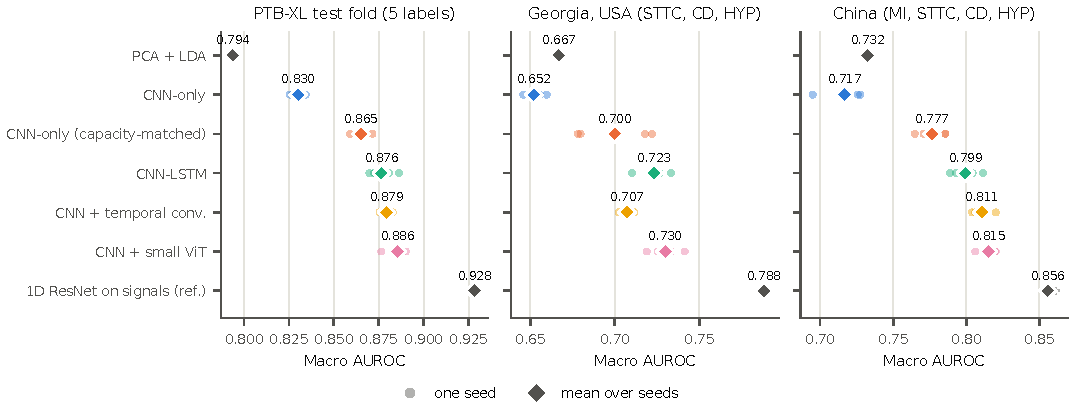
\includegraphics[width=\textwidth]{fig3_head_comparison.pdf}
\caption{Macro AUROC per training seed (light points) and mean over seeds (diamonds) for each model with adaptive-gain pages, on the PTB-XL test fold and the two external cohorts. Macro AUROC is computed over the labels eligible in each cohort.}
\label{fig:heads}
\end{figure}

\subsection*{Adaptive gain is a diagnostic cue}
Because HYP prevalence varied 18-fold across gain levels, the layout of an adaptive-gain page carries information about hypertrophy. Re-rendering the test pages at fixed gain, without retraining, reduced macro AUROC for every adaptive-gain model, slightly for the networks ($-0.002$ to $-0.008$) and strongly for PCA+LDA ($-0.043$ [$-0.054$, $-0.033$]). Predictions on pages whose gain did not change were unaffected (maximum change $1.2\times10^{-5}$).

Integrated gradients located part of the HYP evidence in the calibration pulse (Fig.~\ref{fig:pulse}a). For HYP-positive ECGs, the share of HYP attribution falling on the pulse, which covers 3.6\% of the input width, was 5.3\% for CNN-only, 7.6\% for the temporal-convolution head, 11.4\% for the LSTM and 24.7\% [23.8, 25.5] for the ViT. After fixed-gain retraining, it dropped to 1.4--3.2\%. Swapping only the pulse for a 2.5-mm/mV pulse raised the mean HYP probability of adaptive-gain models by $+0.49$ (ViT), $+0.31$ (LSTM), $+0.15$ (temporal convolution) and $+0.04$ (CNN-only), but changed fixed-gain models by at most 0.014.

A pulse-only swap alters the voltage implied by the page, so these responses mix two mechanisms: a learned prior that a small-gain page signals hypertrophy, and reading the pulse as a voltage scale, as a cardiologist does. The post-hoc decomposition (Fig.~\ref{fig:pulse}b) attributes only $+0.03$ to $+0.08$ to the gain prior. The remainder, up to $+0.46$ for the ViT, reflects calibration reading, which is available only to heads that can relate the pulse to the waveform across the row.

\begin{figure}[!t]
\centering
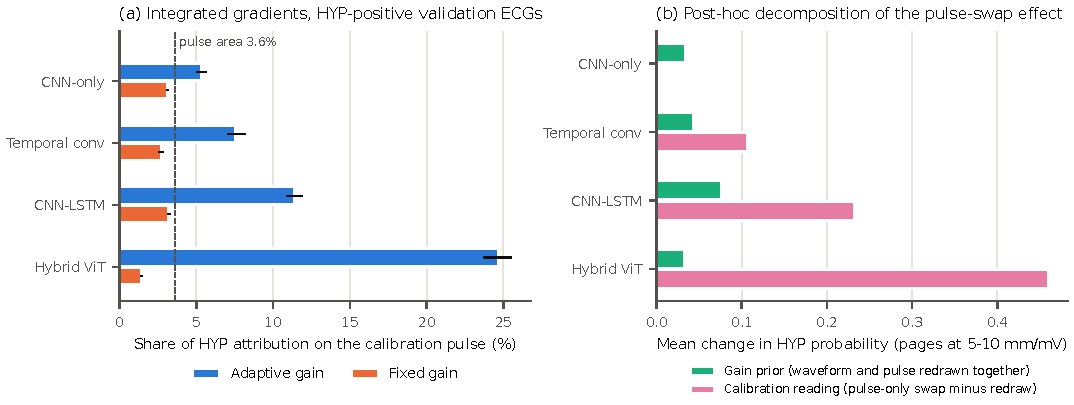
\includegraphics[width=\textwidth]{fig5_calibration_pulse.pdf}
\caption{Use of the calibration pulse (validation, seed 42). (a) Share of integrated-gradients attribution for the HYP logit that falls on the calibration-pulse columns, for HYP-positive ECGs (bars, mean; lines, 95\% patient-bootstrap CI); dashed line, pulse share of the input width. (b) Post-hoc decomposition of the HYP probability change after swapping in a 2.5-mm/mV pulse on pages originally drawn at 5--10~mm/mV: change under consistent re-rendering (gain prior) and the remaining difference (calibration reading).}
\label{fig:pulse}
\end{figure}

\subsection*{Gain-controlled retraining}
On PTB-XL, fixed-gain training raised the macro and HYP AUROC point estimates of every architecture (Table~\ref{tab:fixed}, Fig.~\ref{fig:fixed}), with the largest gains for heads that cannot read the pulse across the row: CNN-only $+0.030$ macro and $+0.073$ HYP AUROC, and temporal convolution $+0.016$ and $+0.043$. Gains were smaller for the LSTM ($+0.012$, adjusted $p=0.028$; HYP $+0.014$, $p=0.11$) and not significant for the ViT ($+0.006$ and $+0.010$, adjusted $p=0.26$). No architecture was worse with fixed gain, and the GPU-only seed set gave the same pattern. With fixed gain, the temporal-convolution head reached the highest image-model test macro AUROC (0.895 $\pm$ 0.001; Table~\ref{tab:ptbxl}). For PCA+LDA, fixed gain lowered macro AUROC (0.794 to 0.781) while raising HYP AUROC (0.820 to 0.837), consistent with smaller deflections being harder to resolve for a linear model on pooled pixels.

\begin{table}[!t]
\centering
\caption{Fixed-gain minus adaptive-gain training: difference in mean-over-seeds AUROC [95\% CI] and Holm-adjusted $p$ (seeds 42--46).}
\label{tab:fixed}
\resizebox{\textwidth}{!}{%
\begin{tabular}{llcccccc}
\toprule
& & \multicolumn{2}{c}{PTB-XL test} & \multicolumn{2}{c}{Georgia, USA} & \multicolumn{2}{c}{Chapman-Shaoxing + Ningbo, China} \\
\cmidrule(lr){3-4}\cmidrule(lr){5-6}\cmidrule(lr){7-8}
Architecture & AUROC & Difference & $p$ & Difference & $p$ & Difference & $p$ \\
\midrule
CNN-only & macro & +0.030 [+0.021, +0.039] & $<$0.001 & +0.055 [+0.045, +0.065] & $<$0.001 & +0.051 [+0.035, +0.071] & $<$0.001 \\
 & HYP & +0.073 [+0.050, +0.098] & $<$0.001 & +0.129 [+0.109, +0.150] & $<$0.001 & +0.112 [+0.088, +0.140] & $<$0.001 \\
\addlinespace[2pt]
CNN + temporal conv. & macro & +0.016 [+0.011, +0.021] & $<$0.001 & +0.031 [+0.023, +0.039] & $<$0.001 & +0.014 [+0.004, +0.023] & 0.018 \\
 & HYP & +0.043 [+0.028, +0.058] & $<$0.001 & +0.096 [+0.078, +0.117] & $<$0.001 & +0.033 [+0.023, +0.045] & $<$0.001 \\
\addlinespace[2pt]
CNN-LSTM & macro & +0.012 [+0.004, +0.021] & 0.028 & +0.015 [+0.007, +0.024] & $<$0.001 & +0.018 [+0.005, +0.031] & 0.012 \\
 & HYP & +0.014 [+0.001, +0.027] & 0.108 & +0.027 [+0.011, +0.045] & $<$0.001 & +0.035 [+0.024, +0.046] & $<$0.001 \\
\addlinespace[2pt]
CNN + small ViT & macro & +0.006 [$-$0.003, +0.013] & 0.256 & +0.008 [+0.004, +0.011] & $<$0.001 & +0.004 [$-$0.004, +0.012] & 0.363 \\
 & HYP & +0.010 [$-$0.003, +0.023] & 0.256 & +0.018 [+0.001, +0.035] & 0.030 & +0.014 [+0.003, +0.026] & 0.018 \\

\bottomrule
\end{tabular}}\\[2pt]
\begin{minipage}{0.95\textwidth}\scriptsize
Macro AUROC over the eligible labels of each cohort; HYP, hypertrophy AUROC. Holm correction over the eight comparisons within each cohort. The PTB-XL comparison uses the same hierarchical bootstrap as the external hypothesis H2; PTB-XL seed 42 pairs a CPU-trained adaptive model with a GPU-trained fixed-gain model.
\end{minipage}
\end{table}

\begin{figure}[!t]
\centering
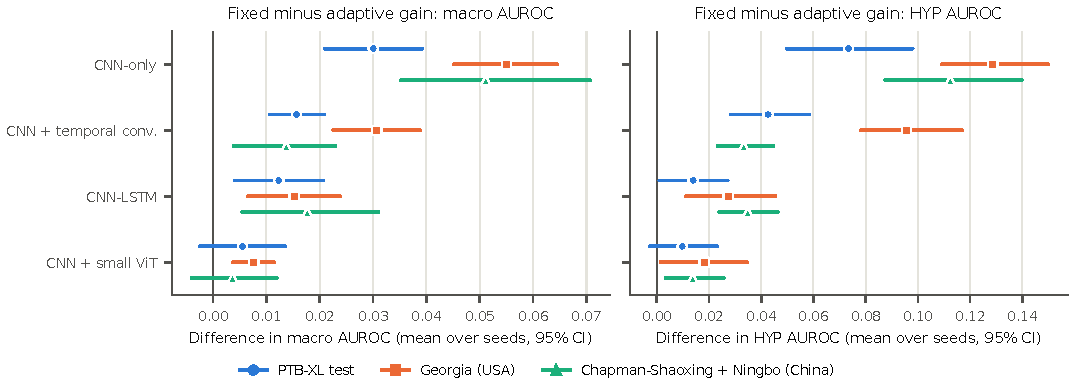
\includegraphics[width=\textwidth]{fig4_fixed_vs_adaptive_gain.pdf}
\caption{Effect of fixed-gain rendering: fixed-gain minus adaptive-gain AUROC (mean over seeds 42--46, 95\% hierarchical bootstrap CI) on the PTB-XL test fold and the two external cohorts, for macro AUROC (left) and hypertrophy AUROC (right).}
\label{fig:fixed}
\end{figure}

\subsection*{External validation}
In Georgia, 6{,}047 of 10{,}344 records were included (52 shorter than 10~s; 4{,}245 without a mapped superclass), with STTC, CD and HYP eligible (MI had 7 positives). In China, 9{,}004 of 45{,}152 were included (2 checksum failures; 36{,}146 without a mapped superclass), with MI, STTC, CD and HYP eligible. NORM was not evaluable in either cohort.

All models lost discrimination out of distribution (Table~\ref{tab:external}; H3): $-0.12$ to $-0.17$ macro AUROC in Georgia and $-0.03$ to $-0.10$ in China, relative to PTB-XL on the same labels.

\emph{H1.} The ordering CNN-only $<$ capacity-matched $<$ \{LSTM, ViT\} replicated in both cohorts with Holm-adjusted $p<0.001$ (Table~\ref{tab:pairs}, Fig.~\ref{fig:heads}). The ViT was the best image model with adaptive gain in both cohorts. The temporal-convolution head was unstable: in Georgia it did not differ from the capacity-matched head and fell below the LSTM ($-0.016$) and ViT ($-0.023$); in China it was tied with the ViT.

\emph{H2.} Fixed-gain training improved HYP AUROC for every architecture in both cohorts, and macro AUROC for every architecture except the ViT in China ($+0.004$, adjusted $p=0.36$; Table~\ref{tab:fixed}, Fig.~\ref{fig:fixed}). The gains were again largest for CNN-only (Georgia $+0.055$ macro and $+0.129$ HYP; China $+0.051$ and $+0.112$). With fixed gain, the three sequence heads were indistinguishable externally (Georgia 0.737--0.738; China 0.817--0.824).

The signal reference remained best (Georgia 0.788; China 0.856), about 0.05 and 0.03 above the best image models.

\begin{table}[!t]
\centering
\caption{External macro AUROC (mean $\pm$ SD over seeds) and difference from PTB-XL test on the same labels ($\Delta$).}
\label{tab:external}
\small
\begin{tabular}{llcccc}
\toprule
& & \multicolumn{2}{c}{Georgia, USA} & \multicolumn{2}{c}{China} \\
\cmidrule(lr){3-4}\cmidrule(lr){5-6}
Pages & Model & AUROC & $\Delta$ & AUROC & $\Delta$ \\
\midrule
Adaptive & CNN-only & 0.652 $\pm$ 0.005 & $-$0.171 & 0.717 $\pm$ 0.013 & $-$0.099 \\
Adaptive & CNN-only, capacity-matched & 0.700 $\pm$ 0.021 & $-$0.162 & 0.777 $\pm$ 0.009 & $-$0.078 \\
Adaptive & CNN-LSTM & 0.723 $\pm$ 0.008 & $-$0.152 & 0.799 $\pm$ 0.009 & $-$0.067 \\
Adaptive & CNN + temporal conv. & 0.707 $\pm$ 0.004 & $-$0.165 & 0.811 $\pm$ 0.006 & $-$0.058 \\
Adaptive & CNN + small ViT & 0.730 $\pm$ 0.008 & $-$0.154 & 0.815 $\pm$ 0.006 & $-$0.062 \\
\midrule
Fixed & CNN-only & 0.707 $\pm$ 0.006 & $-$0.154 & 0.768 $\pm$ 0.011 & $-$0.081 \\
Fixed & CNN-LSTM & 0.738 $\pm$ 0.004 & $-$0.150 & 0.817 $\pm$ 0.007 & $-$0.063 \\
Fixed & CNN + temporal conv. & 0.738 $\pm$ 0.006 & $-$0.154 & 0.824 $\pm$ 0.008 & $-$0.062 \\
Fixed & CNN + small ViT & 0.737 $\pm$ 0.007 & $-$0.152 & 0.819 $\pm$ 0.005 & $-$0.064 \\
\midrule
Adaptive & PCA + LDA & 0.667 & $-$0.125 & 0.732 & $-$0.054 \\
Adaptive & PCA + linear SVM & 0.667 & $-$0.124 & 0.730 & $-$0.056 \\
\midrule
Fixed & PCA + LDA & 0.660 & $-$0.126 & 0.752 & $-$0.025 \\
\midrule
Signal & 1D ResNet (signal) & 0.788 $\pm$ 0.001 & $-$0.132 & 0.856 $\pm$ 0.005 & $-$0.068 \\

\bottomrule
\end{tabular}
\end{table}

\subsection*{Calibration and thresholds}
On the PTB-XL test fold, all models were reasonably calibrated: mean test macro ECE was 0.026 for CNN-only, 0.026 for the LSTM, 0.033 for temporal convolution and 0.046 for the ViT, which over-predicted HYP. Choosing each label's threshold on the validation fold raised the test macro F1 of every model, for example from 0.490 to 0.602 for CNN-only and from 0.666 to 0.684 for the ViT. The fixed threshold of 0.5 therefore understates achievable F1 for rare labels.

\section*{Discussion}
\emph{Sequence modeling versus capacity.} Most of the advantage of sequence heads over simple pooling came from head capacity, but a consistent residual of 0.011--0.020 macro AUROC on PTB-XL, and 0.023--0.039 for the LSTM and ViT externally, required relating columns across the row. Among the sequence heads, no architecture was reliably best on PTB-XL. Externally, attention and recurrence were more robust than local temporal convolution with adaptive gain, but this advantage disappeared once gain was fixed. Model-ranking claims based on a single seed or a single test fold should therefore be treated with caution.

\emph{Gain policy as a hidden variable.} Adaptive gain is a reasonable printing convention, but it turns amplitude into a page-level feature. Our analyses separate two consequences. The gain prior, a learned association between small-gain pages and hypertrophy, is a dataset artifact in the sense of shortcut learning \cite{geirhos2020shortcut}, but its effect on predictions was small ($+0.03$ to $+0.08$ in HYP probability). Calibration reading is legitimate and clinically meaningful, but it is accessible only to architectures with row-wide context. A fixed gain removes the need for it by making pixel amplitude proportional to voltage on every page. This explains why fixed gain helped local heads most, why the attention model's large reliance on the pulse vanished, and why the improvement carried over to unseen cohorts, where amplitude distributions, devices and label practices differ. In practice, the gain policy of a rendered ECG dataset should be fixed, or at least reported and varied, and test sets should be stratified by gain.

\emph{Generalization and the image representation.} All models, including the signal reference, lost substantial discrimination on the external cohorts. Population, device and labeling differences, and a deliberately conservative label mapping (for example, T-wave abnormality fell just below the 90\% rule), all contribute \cite{reyna2022issues}. The persistent advantage of the signal model shows that compact image models still lose information relative to the native waveform, although the comparison also includes a large difference in capacity.

\emph{Limitations.} First, all pages, including the external ones, were clean synthetic renderings; real scans and photographs add artifacts that we did not study \cite{shivashankara2024ecgimagekit,reyna2024challenge}. Second, the models were intentionally small ($\le$24k parameters) to enable a controlled comparison; conclusions about large pretrained image models require separate study. Third, NORM could not be evaluated externally, and MI could not be evaluated in Georgia; external labels come from a data-driven mapping rather than relabeling by cardiologists. Fourth, the PTB-XL test fold had been inspected before the models were specified. Fifth, seed 42 of the four original networks was trained on a CPU and all other runs on a GPU; GPU training is not bit-reproducible, although GPU-only analyses agreed. Sixth, many runs selected their checkpoint in the last epochs of the fixed 20-epoch budget, which may limit some models. Seventh, the pulse-swap decomposition was specified post hoc. Finally, this is a methodological study without clinical evaluation.

\emph{Conclusion.} In a controlled comparison on rendered 12-lead ECG images, heads that relate information along each lead row outperformed a capacity-matched head without sequence mixing, and the ordering largely replicated on independent cohorts from the USA and China. The page gain policy was a first-order design variable: amplitude-dependent gain leaked hypertrophy information and made amplitude-based diagnosis depend on reading the calibration pulse. Fixed-gain rendering removed both effects and improved every architecture on unseen data. ECG-image datasets and benchmarks should fix or explicitly control the gain, and image-model comparisons should report multiple seeds and external tests.

\section*{Methods}

\subsection*{Data and labels}
PTB-XL v1.0.3 \cite{wagner2020ptbxl,wagner2022ptbxl103,goldberger2000physionet} contains 21{,}799 ten-second 12-lead ECGs from 18{,}869 patients, sampled at 500~Hz and annotated by cardiologists with SCP-ECG statements. We used the five diagnostic superclasses (normal ECG, NORM; myocardial infarction, MI; ST/T change, STTC; conduction disturbance, CD; hypertrophy, HYP) as overlapping binary labels, derived with PTB-XL's own statement table. The cohort comprised the 21{,}388 records (18{,}617 patients) with at least one superclass. We used the official patient-disjoint folds: folds 1--8 for training (17{,}084 ECGs), fold 9 for validation (2{,}146) and fold 10 for testing (2{,}158). Fold 10 had been inspected for earlier models before the present models were specified; all PTB-XL test results are therefore labeled exploratory, and the external test (see ``External confirmatory test'' below) is the confirmatory analysis.

\subsection*{Page rendering}
\begin{figure}[!t]
\centering
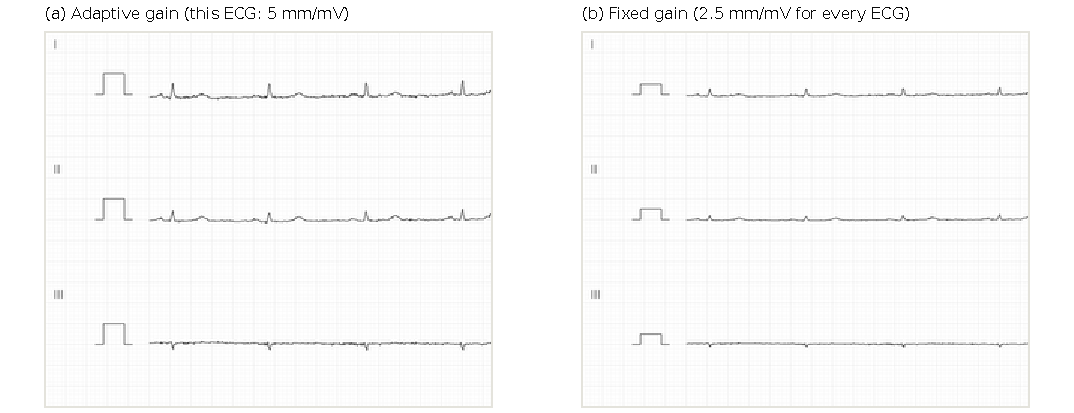
\includegraphics[width=\textwidth]{fig1_rendered_pages.pdf}
\caption{The same PTB-XL ECG (ecg\_id 1; leads I--III, first $\approx$3~s) rendered with (a) the adaptive gain policy, which drew this ECG at 5~mm/mV, and (b) fixed gain (2.5~mm/mV for every ECG). Each row starts with a 1-mV calibration pulse drawn at the page gain.}
\label{fig:pages}
\end{figure}

Each ECG was rendered deterministically as a clean grayscale page at 8~pixels/mm and 25~mm/s: twelve stacked 30-mm rows (leads I--V6), each showing the full 10~s of one lead on a 1-mm/5-mm grid, preceded by a 1-mV, 0.2-s calibration pulse drawn at the same gain as the waveform (Fig.~\ref{fig:pages}). No identifiers, demographics or diagnoses were printed. The page is 2240$\times$3024 pixels. Model inputs were obtained by inverting the intensity, keeping the twelve lead rows and applying 2$\times$2 max pooling, giving a 12$\times$120$\times$1120 ``ink'' tensor per ECG. In model-input columns, the calibration pulse occupies columns 48--87 (3.6\% of the width) and the waveform columns 100--1099.

\emph{Adaptive gain (original renderer).} The nominal gain is 10~mm/mV. Whenever any sample would exceed the 12-mm half-height of a row, the page-wide gain is halved until all samples fit. The gain is printed in the page header and reflected in the calibration pulse height. In PTB-XL, 1{,}456 ECGs were drawn at 10~mm/mV, 14{,}447 at 5, 5{,}135 at 2.5 and 350 at $\le$1.25~mm/mV. HYP prevalence in the training folds rose steeply with decreasing gain: 2.1\% at 10, 6.3\% at 5, 30.8\% at 2.5 and 38.0\% at $\le$1.25~mm/mV. Gain alone, without any image, predicted HYP with AUROC 0.741 (validation) and 0.719 (test).

\emph{Fixed gain.} To remove this cue, every page was re-rendered at 2.5~mm/mV with otherwise identical code; samples beyond a row's limits were clipped at the row edge and counted (154 of 21{,}388 pages; none excluded). Pages already at 2.5~mm/mV in the original rendering were verified to be pixel-identical.

\subsection*{Models}
\begin{figure}[!t]
\centering
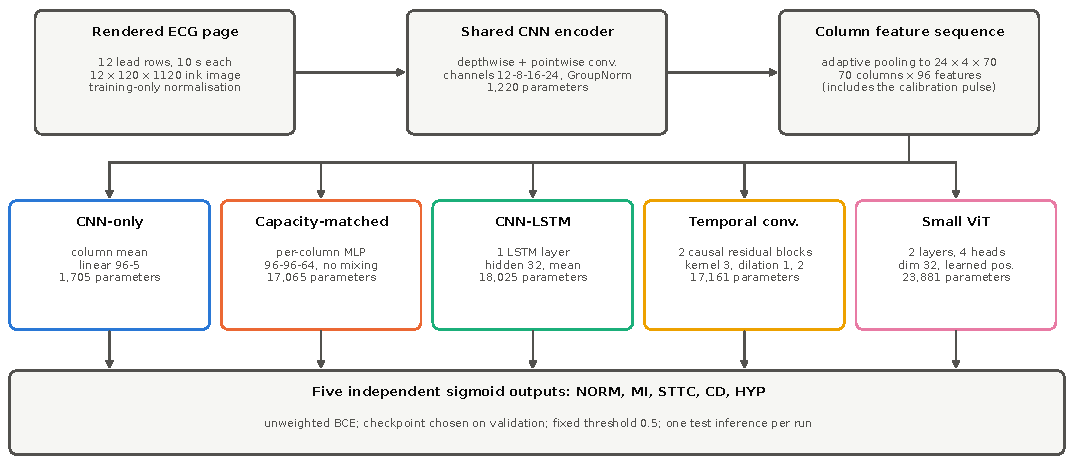
\includegraphics[width=\textwidth]{fig2_architectures.pdf}
\caption{Controlled model design. All networks share the same encoder architecture and column feature sequence and differ only in the head. The capacity-matched head has the parameter budget of the sequence heads but applies the same perceptron to every column separately. References outside the controlled comparison: PCA + LDA and PCA + linear SVM on pooled ink, and a one-dimensional ResNet on the raw signals.}
\label{fig:arch}
\end{figure}

All networks share the same convolutional encoder architecture (Fig.~\ref{fig:arch}), trained from scratch in each run: a lead-wise (depthwise) 5$\times$5 convolution with stride (2,~4) and three depthwise-separable stages, each a depthwise then a pointwise convolution followed by GroupNorm and ReLU (channel widths 12--8--16--24; 1{,}220 parameters), and adaptive average pooling to a sequence of 70 columns with 96 features each (24 channels $\times$ 4 vertical bands). The heads differ only in how this column sequence is aggregated:
\begin{itemize}
\item \emph{CNN-only}: mean over columns, dropout and a linear layer (1{,}705 parameters in total).
\item \emph{Capacity-matched CNN-only}: a two-layer perceptron (96--96--64, ReLU, dropout) applied to every column independently, followed by the column mean and a linear layer (17{,}065 parameters). No operation mixes columns before the mean, so this head cannot relate the calibration pulse, or any part of a row, to another part.
\item \emph{CNN-LSTM}: one unidirectional LSTM layer \cite{hochreiter1997lstm} with 32 hidden units, mean over outputs (18{,}025 parameters).
\item \emph{CNN + temporal convolution}: a 1$\times$1 projection to 32 channels and two causal residual blocks with kernel size 3 and dilations 1 and 2, with LayerNorm (receptive field 13 columns; 17{,}161 parameters) \cite{bai2018tcn}.
\item \emph{CNN + small ViT}: a linear projection to 32 dimensions, learned position embeddings and two transformer encoder layers with four heads and feed-forward width 64 \cite{vaswani2017attention,dosovitskiy2021vit}, followed by LayerNorm and the token mean (23{,}881 parameters).
\end{itemize}
As references outside the controlled comparison, we trained (i) PCA followed by five binary shrinkage linear discriminant analyses, and PCA followed by calibrated linear support vector machines, on 8$\times$8 area-pooled ink (25{,}200 features), with the number of components and the regularization chosen on validation; and (ii) a one-dimensional residual network \cite{wang2017timeseries,he2016resnet} on the raw 100-Hz signals (12$\times$1000; three residual blocks with 64, 128 and 128 channels and kernels 8, 5 and 3; 509{,}573 parameters), with per-lead normalization fitted on the training fold.

\subsection*{Training}
Hyperparameters were fixed before training and shared by all networks: AdamW \cite{loshchilov2019adamw} with learning rate $10^{-3}$ and weight decay $10^{-4}$, batch size 16, at most 20 epochs with cosine annealing to $10^{-5}$ \cite{loshchilov2017sgdr}, dropout 0.2, gradient clipping at norm 1.0, unweighted binary cross-entropy, no augmentation and no pretrained weights. Inputs were standardized with one mean and standard deviation computed on training pixels only. After each epoch, the checkpoint was selected on the validation fold by the lexicographic maximum of (macro AUROC, macro average precision, $-$binary cross-entropy), with early stopping after four epochs without improvement. The decision threshold was fixed at 0.5. Each run performed exactly one test inference, after its checkpoint had been frozen, hashed and reloaded. Every network was trained with seeds 42--46. Seed 42 of the four original networks with adaptive gain (CNN-only, CNN-LSTM, temporal convolution, ViT) was trained on a laptop CPU; all other network runs used an NVIDIA RTX 5070 Ti GPU with deterministic algorithms requested and TF32 disabled (GPU training is not bit-reproducible). Each run records its hardware, and all GPU-only sensitivity analyses are reported.

\subsection*{Evaluation and statistics}
The primary metric was macro AUROC over the five labels. We also report macro average precision, macro F1 at 0.5, per-label AUROC, expected calibration error (ECE, 10 bins) \cite{guo2017calibration} and Brier score. Pairwise head comparisons used a hierarchical bootstrap with 2{,}000 resamples: training seeds were resampled with replacement, then patients (all of their records), both shared by the two models being compared. The statistic was the difference in mean-over-seeds macro AUROC. We report percentile 95\% confidence intervals and two-sided bootstrap $p$-values, $p=2\min\{P(\Delta\le0),P(\Delta\ge0)\}$, adjusted with the Holm procedure within each family (10 head pairs; 8 fixed-versus-adaptive comparisons). An adjusted $p<0.001$ means that no bootstrap replicate crossed zero.

\subsection*{Gain analyses}
\emph{Transfer.} Adaptive-gain models (seed 42) were evaluated once on fixed-gain test pages without retraining. \emph{Retraining.} All networks and PCA+LDA were retrained on fixed-gain pages with identical settings and seeds. \emph{Attribution.} Integrated gradients \cite{sundararajan2017ig} (16 midpoint steps, blank-page baseline) of the HYP logit were summed per input column for 268 HYP-positive and 268 HYP-negative validation ECGs. \emph{Pulse intervention.} On validation pages originally drawn at 5--10~mm/mV (1{,}586 ECGs), the calibration-pulse region was replaced by a pulse drawn at 2.5~mm/mV while the waveform was left unchanged, with sham and masking controls. A post-hoc decomposition, specified after these results were seen, compared this pulse-only swap with the consistent re-rendering of the transfer analysis, in which waveform and pulse change together and the true voltage is preserved.

\subsection*{External confirmatory test}
\emph{Cohorts.} We used the public training sets of the PhysioNet/CinC Challenge 2021 \cite{reyna2021challenge,reyna2022challengedata}: the Georgia 12-lead ECG Challenge database (USA; primary) and the Chapman-Shaoxing \cite{zheng2020chapman} and Ningbo \cite{zheng2022ningbo} databases (China; secondary). The PTB, PTB-XL, CPSC and INCART subsets were not used.

\emph{Plan.} The analysis plan was written and frozen before any external header or signal was parsed; the hashes of the plan and of the label mapping were recorded at the freeze. Inclusion required twelve standard leads at 500~Hz in millivolts, a duration of at least 10~s (the first 10~s were used) and at least one mapped superclass, mirroring the PTB-XL cohort definition.

\emph{Label mapping.} A published PTB-XL-to-SNOMED mapping \cite{strodthoff2023ptbxlplus,strodthoff2023ptbxlplusdata} uses OMOP concept identifiers that do not match the SNOMED CT codes of the Challenge headers. We therefore derived the mapping from the Challenge organizers' own SNOMED CT encoding of PTB-XL. Each header (record HR$xxxxx$ = PTB-XL ecg\_id $xxxxx$) was paired with our PTB-XL labels; age and sex agreed for all 21{,}799 records. A SNOMED code was assigned to a superclass if at least 90\% of the PTB-XL records carrying it had that superclass, among codes present on at least 10 records. This rule was fixed before the mapping was computed and assigned 25 of 50 codes. NORM received no code, because the organizers encoded PTB-XL ``normal ECG'' as sinus rhythm (NORM share 0.53). Labels with fewer than 50 positives or negatives in a cohort were excluded from that cohort's macro AUROC by a prespecified rule.

\emph{Procedure.} External records were rendered with the unchanged adaptive and fixed-gain renderers. Every model of every completed run (52 runs) was first reloaded and verified to reproduce its saved PTB-XL validation probabilities (maximum absolute difference $\le1.5\times10^{-5}$ for every run except the CPU-trained ViT, $4.3\times10^{-4}$). Each run then performed exactly one inference per cohort, using its PTB-XL training normalization and no recalibration. Because the external cohorts lack patient identifiers, records were resampled in the bootstrap. Hypotheses were: H1, the PTB-XL head ordering replicates (10 pairs); H2, fixed-gain training is not worse than adaptive-gain training for any architecture (macro and HYP AUROC; 8 comparisons); H3, the external-minus-PTB-XL difference (descriptive). Two Ningbo signal files never matched PhysioNet's published SHA-256 over three download attempts and were excluded by a dated amendment recorded before any Chinese header was read.

\section*{Data availability}
PTB-XL and the PhysioNet/CinC Challenge 2021 data are publicly available on PhysioNet under the Creative Commons Attribution 4.0 license. The code, frozen configurations and protocols, run records (configuration, code hashes and snapshots, saved predictions and metrics) and analysis scripts will be released in a public repository upon publication [link to be added].

\bibliography{references}

\section*{Acknowledgements}
[To be completed by the authors, including funding.]

\section*{Author contributions}
[To be completed by the authors.]

\section*{Competing interests}
[To be completed by the authors.]

\end{document}
